%!TEX root = ../dokumentation.tex

\chapter{Rahmenbedingungen}


\section{Export-Datenstruktur}

Wie bereits im Kapitel zuvor erwähnt bietet Kubios HRV Premium zwei unterschiedliche Exportmöglichkeiten. Diese werden durch den einheitlichen CSV-Standard und das MATLAB-eigenen MAT-File repräsentiert.\\
Bei einer CSV-Datei (engl. Comma-separated values) handelt es sich um einen Standard, welcher den Aufbau einer Textdatei beschreibt. Der Inhalt der Datei beschränkt sich meist auf Tabellen und Listen, welche nicht wie üblicherweise in Zeilen und Spalten aufgeteilt wird, sondern mit Hilfe von Kommas getrennt wird, wobei jede neue Zeile eine neue Datenbankzeile darstellt und jede Datenbankzeile aus einem oder mehreren Feldern besteht. CSV-Dateien finden vor allem Anwendung in Tabellenkalkulationsprogrammen und Datenbanksysteme, wie Microsoft Excel oder MySQL, welche das Format einlesen, sowie exportieren können. Aufgrund der weiten Verbreitung des Formats ist auch das Einlesen und Verarbeiten der Dateien in nahezu jeglicher Programmiersprache möglich. Vor allem Python bietet passende Bibliotheken und Funktionen.\\% https://datei.wiki/extension/csv
Das MAT-File beschreibt ein binäres Datencontainerformat, welches von MATLAB verwendet wird. Es ermöglicht das Speichern von Arrays, Variablen und Funktionen. Je nach MATLAB Version ermöglicht das Format zusätzlich die Speicherung von mehrdimensionale numerische Arrays, Zeichenarrays, Zellenarrays, Felder mit geringer Dichte, Objekte und Strukturen. Die Lesbarkeit beschränkt sich hier jedoch auch auf MATLAB und einige wenige Bibliotheken für beispielsweise Python.
% https://datei.wiki/extension/mat

Da diese beiden Export-Formate und deren Inhalt von einander verschieden sind und die Grundlage der Datenverarbeitung sowie Datenvisualisierung bilden, sollen diese im Folgenden Hinblick auf Übersichtlichkeit, Formatierung, inhaltlicher Korrektheit und Zugänglichkeit verglichen werden.\\
Die Darstellung der CSV-Datei ist unverschachtelt und befindet sich auf einer Ebene. Alle Daten lassen sich auf einmal einsehen. Innerhalb der Datei befinden sich tabellarische Strukturen der einzelnen Messdaten, aber auch Einzelinformationen, Überschriften und Bezeichner. Dies stellt für das Einlesen und Verarbeiten der Daten ein Problem dar, da zusätzlich nach relevanten gefiltert oder mehrere Formatierungsiterationen durchgeführt werden müssen. Das MAT-File hingegen ist in sich verschachtelt. Die Messdaten sind sortiert und unter ihrem jeweiligen Bereich geordnet. Der Zugriff auf die Daten erfolgt mittels Key-Value-Verfahren, das heißt unter einem Schlüsselwort befinden sich der jeweilige Datensatz. Ein Datensatz kann dabei ebenfalls von einem weiteren Key-Value-Paar dargestellt werden. Irrelevante Daten können hier gefiltert werden in dem man den jeweiligen Key einfach nicht aufruft. Das Format kann also ohne weitere Vorformatierung eingelesen werden.\\
Betrachtet man die Konstanz und Korrektheit bezogen auf die Darstellung der Daten in Kubios, lassen sich im CSV-Format einige Unregelmäßigkeiten erkennen. So sind häufig Kommas verschoben und Felder mit einer stark variierenden Anzahl Leerzeichen aufgefüllt, um eine übersichtlichere Darstellung zu ermöglichen. Dies hat jedoch den Effekt, dass diese Leerzeichen beim Einlesen mit beispielsweise Python ebenfalls im Datensatz auftauchen und diesen verunreinigen bzw. im schlimmsten Fall unbrauchbar machen. Auch hier müsste deshalb im Vorhinein ein Formatierung der grundlegenden Datei durchgeführt werden. \color{red}Diese Unregelmäßigkeiten lassen sich auf die Exportfunktionen der Kubios-Software zurückführen. \color{black}Der Inhalt des MAT-Files ist hingegen akkurat und nicht von den Unregelmäßigkeiten betroffen.

Daraus ergibt sich, dass das MAT-File ein grundlegend konsistenterer Datenspeicher für die medizinischen Messdaten darstellt und einen großen Vorteil im Bereich der Zugänglichkeit sowie der Reduzierung zusätzlicher Hilfsfunktionen und Datenmanipulationen gegenüber dem CSV-Format bietet. Aus diesem Grund wird dieses auch als Grundlage zur Umsetzung des Tools zur Auswertung der medizinischen Messdaten verwendet.


\section{Programmiersprache}

Im Bereich der Data Science gibt es viele unterschiedliche Programmiersprachen, welche das Bearbeiten und Auswerten großer Datenmengen ermöglichen. Je nach Anwendungsgebiet und Lösungsansätzen, sowie der dazugehörigen Eigenschaften der zu analysierenden Daten muss eine passende Programmiersprache gewählt werden. Im Hinblick auf die Anforderungen der Studienarbeit stehen vor allem das Auslesen der Daten aus vorgegebenen Datei-Formaten, das graphische Darstellen der Messdaten, sowie die Erstellung einer passenden Benutzeroberfläche im Vordergrund. 

Python ist hierbei die beliebteste und meistverwendet Programmiersprache. Sie ermöglicht das effiziente Auslesen von CSV-Datei sowie MAT-Dateien, verfügt über die Möglichkeit eine Benutzeroberfläche zu erstellen und bietet mit einer großen Anzahl zusätzlicher Bibliothek eine hohe Flexibilität. Somit ist Python perfekt auf die Anforderungen der Aufgabenstellung zugeschnitten. Da die Messdaten jedoch in der zukünftigen Implementierung aus der MAT-Datei ausgelesen werden sollen, wird auch die Umsetzung in MATLAB betrachtet. MATLAB bietet dabei auch eine Reihe von Tools zum Auswerten verschiedener Daten und das erstellen einer graphische Benutzeroberfläche. Beide Programmiersprachen stellen alle benötigten Funktionen sowie Ansätze zur Lösung der Aufgabenstellung dar und werden häufig direkt miteinander verglichen, da die Überschneidung ihrer Anwendungsgebiete sehr groß ist. Um eine Entscheidung über die zu verwendende Programmiersprache treffen zu können werden diese im folgenden vorgestellt und anhand wichtiger Kriterien miteinander verglichen.

\subsection{Python}

Python ist eine interpretierte, objektorientiere High-Level-Programmiersprache mit einer dynamischen Semantik, welche in den Bereichen der Datenanalyse und Machine Learning, aber auch im Web Development oder für Automatisierungstasks eingesetzt wird. Sie glänzt vor allem durch ihre hochentwickelten, integrierten Datenstrukturen und dynamischer Typisierung, weshalb sie sehr attraktiv für Anwendungs- sowie Skriptentwicklung ist. Auch die einfache und leicht zu erlernende Syntax von Python, bietet einen guten Einstieg in die Programmierung, beschleunigt den Entwicklungsprozess und erleichtert die Programmpflege. Außerdem unterstützt Python eine Großzahl von Modulen und Paketen, was die Modularität von Programmen und die Wiederverwendung von Code fördert. Diese werden vor allem auch durch die große Community und deren Open-Source-Projekte weiter gefördert, weshalb grundlegende Lösungen für nahezu jedes Problem bereits bestehen. Der Python-Interpreter und die umfangreiche Standardbibliothek sind für alle wichtigen Plattformen kostenlos verfügbar und können frei verteilt werden.

% https://www.python.org/doc/essays/blurb/
% https://www.coursera.org/articles/what-is-python-used-for-a-beginners-guide-to-using-python

\subsection{MATLAB}

MATLAB ist eine High-Level-Prgrammiersprache für technische Berechnungen, welche von \textit{The MathWorks Inc.} entwickelt sowie vertrieben wird und deshalb auch eine kostenpflichtige Lizenz benötigt. Sie integriert Berechnungen, Visualisierung und Programmierung in einer einfach zu bedienenden Umgebung, in der Probleme und Lösungen in vertrauter mathematischer Notation ausgedrückt werden. Ihre Anwendungsgebiete sind dabei mathematische Berechnungen und Algorithmen-Entwicklung, sowie die Simulation und Datenanalyse, aber auch die Entwicklung von Anwendungen, einschließlich der Erstellung von graphischen Benutzeroberflächen sind möglich.\\
MATLAB basiert grundlegend auf einem Array-Datenelement, welches nicht dimensioniert werden muss. Dadurch lassen sich viele technische Berechnungsprobleme, insbesondere solche mit Matrix- und Vektorformulierungen, in einem Bruchteil der Zeit lösen, die für das Schreiben eines Programms in einer skalaren, nicht interaktiven Sprache wie C erforderlich wäre. MATLAB bietet eine Reihe anwendungsspezifischer Lösungen, die so genannten Toolboxen. Toolboxen sind umfassende Sammlungen von MATLAB-Funktionen, die die MATLAB-Umgebung erweitern, um bestimmte Problemklassen zu lösen. Zu den Bereichen, in denen Toolboxen verfügbar sind, gehören Signalverarbeitung, Steuerungssysteme, neuronale Netze, Simulation und viele andere.

% https://de.mathworks.com/discovery/what-is-matlab.html
% https://blog.devgenius.io/what-is-matlab-why-we-need-it-d61e405ef419

\subsection{Performance-Vergleich}

Um einen besseren Überblick über die Performance der beiden Programmiersprachen zur Auswertung von Messdaten zu erhalten, werden mehrere Performance-Vergleiche durchgeführt. Getestet wird auf einem MacBook mit folgenden technischen Daten, welcher sich im Akku-betriebenem Modus befindet. 

\begin{table}[H]
	\centering
	\begin{tabular}{|l|l|}
		\multicolumn{1}{l}{\textbf{Technische Daten}} & \multicolumn{1}{l}{}                       \\ 
		\hline
		Model                                         & MacBook Pro (Retina, 13-inch, Early 2015)  \\ 
		\hline
		Betriebssystem                                & macOS Montery Version 12.1                 \\ 
		\hline
		Prozessor                                     & 2,7 GHz Dual-Core Intel Core i5            \\ 
		\hline
		Arbeitsspeicher                               & 8 GB 1867 MHz DD3                          \\ 
		\hline
		Grafikchip                                    & Intel Iris Graphics 6100 1536 MB           \\
		\hline
	\end{tabular}
	\caption{Übersicht der technischen Daten des Testmediums}
\end{table}

\subsubsection{Analyse anhand der Berechnung einer Regressionsfunktion}

Zuerst wird ein allgemeiner Geschwindigkeitstest durchgeführt. Hierzu soll sowohl in Python als auch in MATLAB die Methode der kleinsten Quadrate (engl. ordinary least squares - kurz OLS) zur Regression anhand eines zufällig generierten Datensatzes durchgeführt werden. Mit Hilfe von Ausgleichsrechnungen kann eine möglichste genau passende, modellabhängige Modellkurve in eine Wolke von Datenpunkten gelegt werden. In der Methode der kleinsten Quadrate wird die Summe der quadratischen Abweichungen der Kurve von den beobachteten Punkten minimiert. Ausgleichsrechnungen sind ein wichtiger Bestandteil der Datenanalyse und sind größtenteils rechenintensiv wenn sie auf große Datenmengen angewendet werden, deshalb bietet diese Methode ein gutes Beispiel zum Vergleich der Programmiersprachen und ihrer Performance. 
% https://mathepedia.de/Methode_der_kleinsten_Quadrate.html

Die Methode der kleinsten Quadrate wurde mit einer Replikation von 1000 durchgeführt. Für die Erstellung des Beispieldatensatzes werden die folgenden wahren Parameter verwendet.

\begin{equation}
	\beta = \begin{bmatrix}
	 	10\\ 
	 	-0,5\\ 
	 	0,5
	\end{bmatrix}
\end{equation} 

Die Regression wird für drei unterschiedliche Datensatzgrößen mit n = 1000, 10000 und 100000 umgesetzt. Für jede Beobachtung werden die unabhängigen Variablen aus folgenden Werten gezogen:

\begin{equation}
	\mu _{x} = \begin{bmatrix}
		10\\ 
		10
	\end{bmatrix}
	, \sigma _{x} = \begin{bmatrix}
		4 & 0\\ 
		0 & 4
	\end{bmatrix}
\end{equation} 

Die abhängige Variable wird konstruiert, indem ein Vektor von zufälligen Normalvariablen aus Normal(0,1) gezogen wird. Dieser Vektor wird als $ \epsilon $ bezeichnet, und die abhängige Variable wird wie folgt berechnet:

\begin{equation}\formelentry{Berechnung der abhängigen Variable - OLS}
	Y = Xb + \epsilon 
\end{equation} 

Für die Berechnung der Parameter werden integrierte Funktionen der beiden Programmiersprachen verwendet. MATLAB basiert hierbei auf der \textbf{OLS-Funktion}, während bei Python die \textbf{statsmodels}-Bibliothek, sowie wie \textbf{numpy} und \textbf{pandas} zur Datenverarbeitung zum Einsatz kommen. Hierbei muss angemerkt werden, dass im folgenden davon ausgegangen wird, dass diese aufgrund ihre Definition als State-of-the-Art bereits auf Geschwindigkeit optimiert sind und eine aussagekräftige Darstellung des Performance-Vergleich bieten können.\\
Für den Vergleich fällt die Beschränkung der Zeitmessung auf das Auswählen von Stichproben aus dem Datensatz, das Berechnen der Parameterschätzung durch OLS und das Abspeichern der Ergebnisse. Die Erzeugung der Datensätze wird hingegen nicht mit in die Zeitmessung aufgenommen. Beide Implementierungen wurden im Vorhinein bereits nach grundlegenden Code-Optimierungen angepasst.

\lstinputlisting[language=Matlab,numbers=left,firstline=1,lastline=21,caption={Methode der kleinsten Quadrate MATLAB Implementierung}]{code/ols_test.m}
\lstinputlisting[language=Python,numbers=left,firstline=1,lastline=30,caption={Methode der kleinsten Quadrate Python Implementierung}]{code/ols_test.py}

\begin{figure}[H]
	\begin{minipage}[b]{.4\linewidth} % [b] => Ausrichtung an \caption
		\begin{table}[H]
			\begin{tabular}{|l|l|l|}
				\hline
				\textbf{n} & \textbf{MATLAB} & \textbf{Python} \\ \hline
				1000       & 0.3571               & 0.3072               \\ \hline
				10000      & 0.6031               & 1.7127               \\ \hline
				100000     & 3.7375               & 21.5871              \\ \hline
			\end{tabular}
			\caption{Zeitmessungen der Datensatzgrößen und Implementierungen}
		\end{table}
	\end{minipage}
	\hspace{.1\linewidth}% Abstand zwischen Bilder
	\begin{minipage}[b]{.4\linewidth} % [b] => Ausrichtung an \caption
		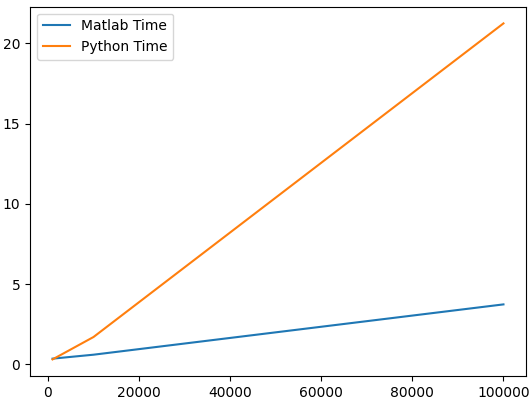
\includegraphics[width=1.25\linewidth]{oslGraph}
		\caption{Visualisierung der Zeitmessung}
	\end{minipage}
\end{figure}

An den Zeitmessung für verschieden große Datensätze lässt sich gut erkennen, dass MATLAB und Python für kleine Datenmengen eine ähnlich große Berechnungszeit benötigen. Mit zunehmender Datenmenge wächst auch die Berechnungszeit. MATLAB skaliert hier jedoch um ein Vielfaches besser und es lässt sich eine stetige steigende Lücke zwischen den Ausführungszeiten erkennen.

% https://rlhick.people.wm.edu/posts/comparing-the-speed-of-matlab-versus-pythonnumpy.html

\subsubsection{Analyse anhand der einfachen Datenvisualisierung}

Im nächsten Schritt soll ein Performance-Test durchgeführt werden, welcher stärker in Richtung der Aufgabenstellung ausgelegt ist. Hierzu wird ein kleiner Datensatz geöffnet und ein einfache Line-Plot erstellt. Geplottet wird jeweils die durchschnittliche Herzfrequenz aus dem normalen Datensatz der Auswertung ohne Samples. Hierbei handelt es sich um 41 Werte, welche als Line-Plot ohne weitere Konfiguration dargestellt werden. In der Python Umgebung werden die Bibliotheken \textbf{pandas} und \textbf{h5py} verwendet, da diese für ihre jeweiligen Aufgaben, Erstellen von Data Frames und Laden von mat-Files, als State-Of-The-Art gelten. Zum Plotten wird auf die \textbf{matplotlib} zurückgegriffen, da diese der MATLAB Darstellung am nächsten kommt. MATLAB ermöglicht die Auswertung ohne zusätzliche Bibliotheken. Die Zeit wird in beiden Fällen mit nativen Funktionen ausgewertet. Die Implementierungen der einzelnen Programmiersprachen, sowie die berechneten Programmlaufzeiten sind im Folgenden dargestellt. Die beiden Skripte werden jeweils fünf mal ausgeführt und der Mittelwert der berechneten Zeiten bestimmt.

% https://pandas.pydata.org/
% https://docs.h5py.org/en/stable/

\lstinputlisting[language=Matlab,numbers=left,firstline=1,lastline=4,caption={Line-Plot MATLAB Implementierung}]{code/speedtest.m}
\lstinputlisting[language=Python,numbers=left,firstline=1,lastline=13,caption={Line-Plot Python Implementierung}]{code/speedtest.py}

\begin{table}[H]
	\centering
	\begin{tabular}{|l|l|l|}
		\multicolumn{1}{l}{\textbf{Durchlauf}} & \multicolumn{1}{l}{\textbf{MATLAB}} & \multicolumn{1}{l}{\textbf{Python}}  \\ 
		\hline
		1                                      & 0.303867 s                          & 0.359526
		s                           \\ 
		\hline
		2                                      & 0.307696
		s                          & 0.351593
		s                           \\ 
		\hline
		3                                      & 0.295474
		s                          & 0.354158
		s                           \\ 
		\hline
		4                                      & 0.301647 s                          & 0.352104 s                           \\ 
		\hline
		5                                      & 0.299218 s                          & 0.350182 s                           \\ 
		\hline
		\textbf{Mittelwert}                    & \textbf{0.301580 s}                          & \textbf{0.353512} s                           \\
		\hline
	\end{tabular}
		\caption{Ergebnisse der Geschwindigkeits-Messungen}
\end{table}

MATLAB ist bei jeder Ausführung um ca. 17\% schneller als das Python Skript. Außerdem muss hier beachtet werden, dass das Anzeigen des Plots unter Python nicht mit in die Berechnung der Zeit aufgenommen werden kann, da alle Code-Zeilen nach \glqq plt.show\grqq{} auch erst nach dem Schließen des Plot-Fensters angezeigt werden. Da die Geschwindigkeit bei kleinen simplen Skripten nicht wirklich aussagekräftig ist, soll hier vor allem das Augenmerk auf die Umsetzung gesetzt werden. Deshalb muss vor allem die Komplexität der beiden Skripte betrachtet werden. In MATLAB benötigt man lediglich zwei Zeilen Code und keine zusätzlichen Bibliotheken, während das Python Skript vier Code Zeilen und drei zusätzlichen Bibliotheken in Anspruch nimmt.

\subsubsection{Fazit und Begründung der Entscheidung}

MATLAB ist für die Umsetzung des Evaluierungs-Tools die schnellere und passendere Programmiersprache. Dies lässt sich vor allem auf die allgemein bessere zeitliche Performance innerhalb mathematischer Berechnungen aber auch beim Einlesen und Visualisieren von Datensätzen zurückführen. Zudem ist die MAT-Datei, welche im späteren Verlauf der Studienarbeit durch Kubios erstellt wird ein nativer Datentyp von MATLAB. Dadurch lässt sich allgemein ein einfacherer Umgang mit den Daten garantieren, sowie die Reduzierung von Code-Komplexität durch einfacher gehaltene Datenverarbeitung ermöglichen. So lässt sich die innere Struktur der MAT-Datei in MATLAB direkt einsehen und es sind keine zusätzlichen Bibliotheken und Funktionen notwendig.

Betrachtet man die Komplexität bezogen auf die Erstellung von Applikationen und das dazugehörigen Design, lässt sich keine objektiv bessere Programmiersprache für die Aufgabenstellung erkennen. Hierbei handelt es sich rein um eine persönliche Präferenz, da die Möglichkeiten beider Sprachen vergleichbar bis gleich sind.